Along with the implementation of the proof-of-concept, multiple experiments were conducted to evaluate the networking and computational performance of the proposed approach. The testbed was empirically hosted on a laptop with an AMD Ryzen 7 4700U CPU and 16 GB of RAM, running an x86-64 Linux 6.1.24-1-lts system. Every instance got assigned 1 GB of RAM and 2 virtual CPUs. 

The bridge interface, pooling all the mesh traffic exchanged between the tap interfaces, was the starting point for the networking measurements. All these interfaces had a maximum virtual bandwidth of 10 Mbit per second, assigned by the hosting system. The traffic was monitored using Wireshark\footnote{\url{https://www.wireshark.org/}}, and the metrics were collected throughout the various stages of the experiment, by listening to packets of different kinds, flowing through the bridge interface. Establishing the mesh network connectivity, the Ethernet frames belonging to the batman-adv protocol sized an average of 74 bytes, and the IPv4 related packets averaged at 278 bytes, presenting both protocols a seemingly linear throughput increase with the increase in the number of instances, as shown in Figure~\ref{fig:mesh-traffic}. 

\begin{figure} [h!]
    \centering
    \begin{subfigure}[b]{0.49\textwidth}
        \centering
        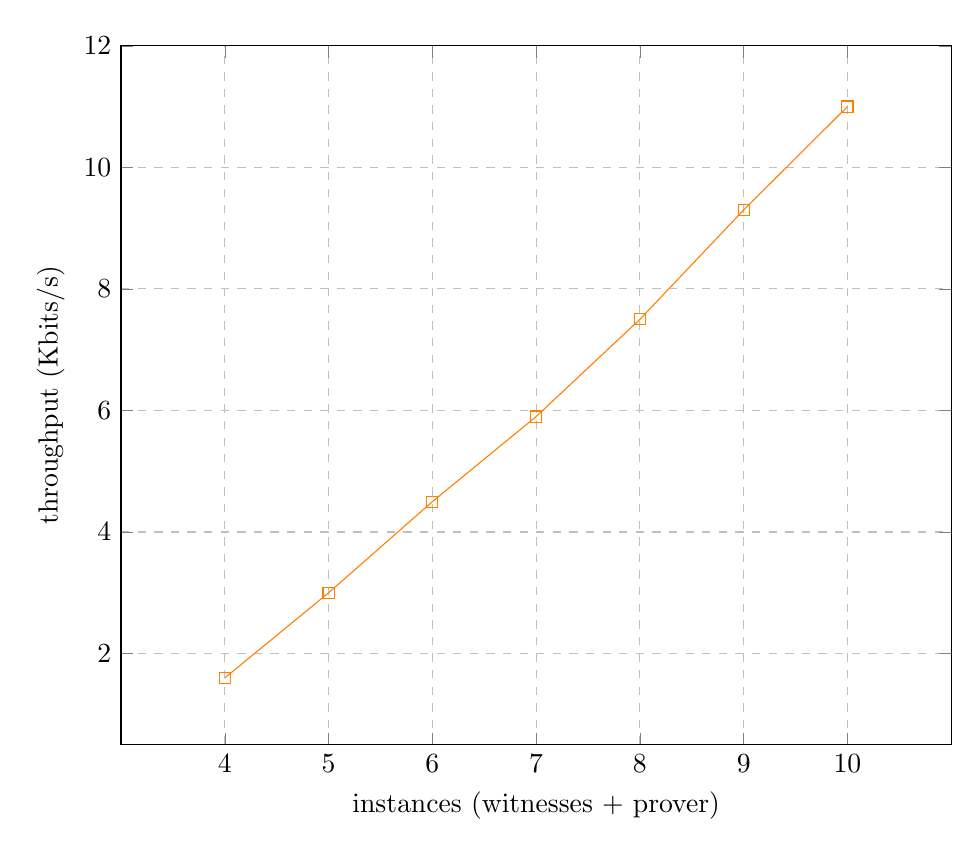
\begin{tikzpicture}
            \definecolor{line-color}{RGB}{92,255,230}
            \definecolor{line-color2}{RGB}{3,150,156}
            \begin{axis}[
                legend pos=outer north east,
                xlabel=instances (witnesses + prover),
                ylabel=throughput (Kbits/s),
                xmin=3, xmax=11,
                ymin=0.5, ymax=12,
                xtick={4,5,6,7,8,9,10},
                ytick={2, 4, 6, 8, 10, 12},
                grid=major,
                grid style={dashed},
                width=\textwidth
            ]
            
            \addplot[color=orange,mark=square] coordinates {
                (4,1.6) (5,3.0) (6,4.5) (7,5.9) (8,7.5) (9,9.3) (10,11)
                % (4,3.4) (5,5.7) (6,8.1) (7,11.2) (8,14) (9,16.8) (10,20)
            };
            \end{axis}
        \end{tikzpicture}
        \caption{Batman-adv traffic throughput.}
        \label{fig:y equals x}
    \end{subfigure}
    \hfill
    \begin{subfigure}[b]{0.49\textwidth}
        \centering
        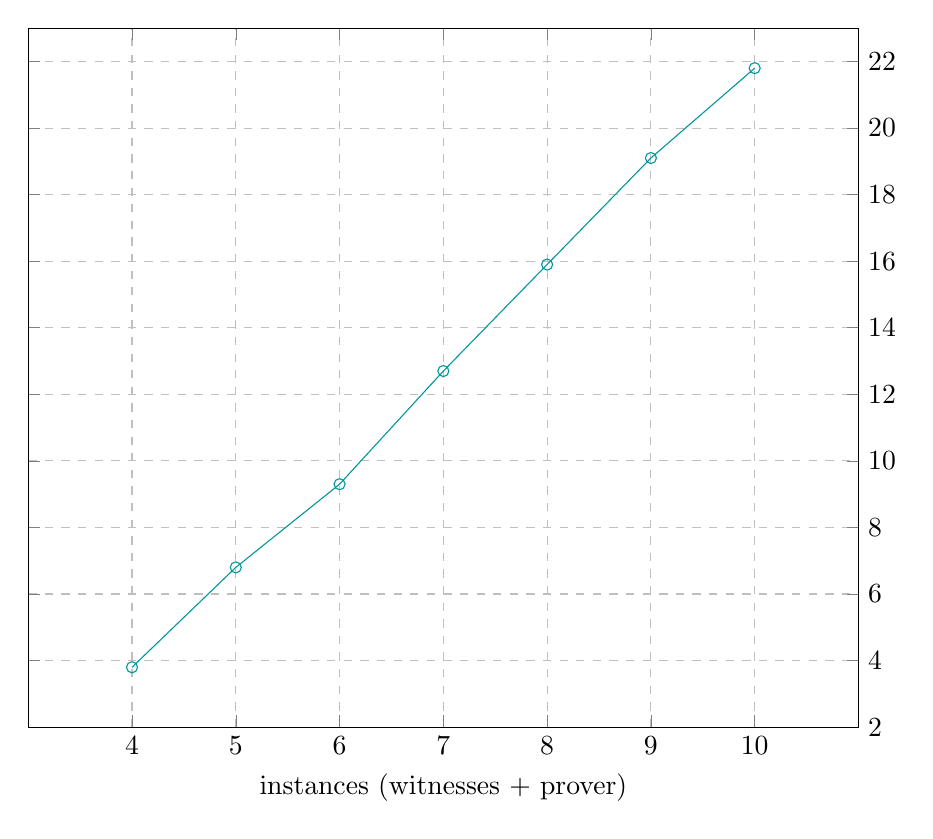
\begin{tikzpicture}
            \definecolor{line-color}{RGB}{92,255,230}
            \definecolor{line-color2}{RGB}{3,150,156}
            \begin{axis}[
                legend pos=outer north east,
                xlabel=instances (witnesses + prover),
                % ylabel=throughput (Kbits/s),
                yticklabel pos=right,
                xmin=3, xmax=11,
                ymin=2, ymax=23,
                xtick={4,5,6,7,8,9,10},
                ytick={2, 4, 6, 8, 10, 12, 14, 16, 18, 20, 22},
                grid=major,
                grid style={dashed},
                width=\textwidth,
            ]
            
            \addplot[color=line-color2,mark=o] coordinates {
                (4,3.8) (5,6.8) (6,9.3) (7,12.7) (8,15.9) (9,19.1) (10,21.8)
            };        
            \end{axis}
        \end{tikzpicture}
        \caption{IPv4 traffic throughput.}
        \label{fig:three sin x}
    \end{subfigure}
    \caption{Average protocol throughput, measured in the bridge interface.}
    \label{fig:mesh-traffic}
\end{figure}

The Blockchain activity was also monitored, in order to observe the protocol behaviour, regarding the block generation and proposal phases. Figure~\ref{fig:blockchain-blocks-generation} captures the number of messages exchanged between the instances, during a time frame of typical protocol activity. The interval time between blocks, set to 10 seconds, corresponds to the higher peaks of TCP traffic, while the UDP traffic is more evenly distributed. This behaviour gets more pronounced as the number of instances increases. 

\begin{figure} [h!]
    \centering
    \begin{subfigure}[b]{\textwidth}
        \centering
        \pgfplotstableread[col sep=comma]{data/blockchain-blocks-generation-4-instances.csv}\datatable
        
        \begin{tikzpicture}
            \definecolor{line-color}{RGB}{3,150,156}
            \definecolor{line-color2}{RGB}{167,169,172}
            \begin{axis}[
                xlabel=time (s),
                ylabel=messages,
                xmin=-2, xmax=102,
                ymin=-5, ymax=40,
                ytick={0, 5, 10, 15, 20, 25, 30, 35, 40},
                grid=major,
                grid style={dashed},
                width=\textwidth,
                height=0.5\textwidth,
                legend pos=north west
            ]
        
            \addplot[mark=*,line-color] table[x=x,y=TCP]{\datatable};
            \addplot[mark=+,line-color2] table[x=x,y=UDP]{\datatable};
            \addplot[mark=o,orange] table[x=x,y=Batman-adv-orig]{\datatable};
        
            \legend{TCP, UDP, Batman-adv-orig}
        
            \end{axis}
        \end{tikzpicture}
        \caption{4 instances.}
        \label{fig:blockchain-blocks-generation-4-instances}
    \end{subfigure}
    \hfill
    \begin{subfigure}[b]{\textwidth}
        \centering
        \pgfplotstableread[col sep=comma]{data/blockchain-blocks-generation-8-instances.csv}\datatable
        
        \begin{tikzpicture}
            \definecolor{line-color}{RGB}{3,150,156}
            \definecolor{line-color2}{RGB}{167,169,172}
            \begin{axis}[
                xlabel=time (s),
                ylabel=messages,
                xmin=-2, xmax=102,
                ymin=-50, ymax=300,
                ytick={0, 50, 100, 150, 200, 250, 300},
                grid=major,
                grid style={dashed},
                width=\textwidth,
                height=0.5\textwidth,
                legend pos=north west
            ]
        
            \addplot[mark=*,line-color] table[x=x,y=TCP]{\datatable};
            \addplot[mark=+,line-color2] table[x=x,y=UDP]{\datatable};
            \addplot[mark=o,orange] table[x=x,y=Batman-adv-orig]{\datatable};
        
            \legend{TCP, UDP, Batman-adv-orig}
        
            \end{axis}
        \end{tikzpicture}
        \caption{8 instances.}
        \label{fig:blockchain-blocks-generation-8-instances}
    \end{subfigure}
    \caption{The network activity, with a block time of 10 seconds.}
    \label{fig:blockchain-blocks-generation}
\end{figure}

Both CPU and RAM usages were also continuously measured across the whole experiment. The two virtual cores of each instance saw the CPU usage averaging at 2\%, peaking at 20\% when the prover would interact with a witness, or vice versa, in order to produce a \pol{} certificate. The overall RAM usage did not go beyond 200 MB. These numbers are in line with the expected behaviour of the protocol, running the PoA consensus algorithm, as a lightweight mechanism that may not require much computational power, suitable and adaptable to resource-constrained environments. The PoW consensus algorithm, on the other hand, would require a much higher and variable computational power, that would be difficult to predict and control, as it is not only manually configured, but dependent, as well, on the dynamic difficulty adjustment mechanism, in order to meet a fixed block time. In terms of storage, the disk space used did not exceed 65 MB, for the entire file system.

The proof generation process did not possess enough relevancy for time measurement purposes. Its execution speed, during the transaction creation, signing, and broadcasting phases is highly dependent on the running environment, and not limited to the showcased implementation. It can be effectively optimized in multiple ways, using different libraries, programming languages, or parallelization techniques. Moreover, the total execution time is ultimately bounded to the block time, as the prover needs to wait a maximum of $T$ units of time for the generation of the new block that may contain its transaction. The proof generation process is also not a bottleneck in the protocol, as it is not a part of the consensus mechanism, and may be executed in parallel with the other protocol activities. The certificate assembly and verification processes can, as well, be performed later and asynchronously. Nonetheless, the success rate of the generation of \pol{} certificates may still be assessed. For such experiment, the interval time between blocks was adjusted and the number of valid \pol{} certificates was measured. A similar test was conducted by Nosouhi et al. \cite{nosouhi2020blockchain}, targeting the effectiveness of their protocol against prover-prover collusions, or proxy and wormhole attacks. The test is still dependent on the characteristics of the running environment, but the results sustain the conclusion that the block time is a crucial parameter in the protocol. Figure~\ref{fig:block-time-success-rate} shows a direct relation between the block time and the success rate in generating valid certificates. The higher the block time, the lower the failures. The consequences of such relation are twofold. A more permissive block time allows for a lower number of invalid certificates, but also for a higher probability of witnessing malicious activity, such as collusions between adversaries and remote provers, as explained in Figure~\ref{fig:pol-implementation:overview-proxy-wormhole}. The block time is, therefore, a trade-off between the two, and should be carefully adjusted to the running environment, in order to achieve the desired levels of security and performance. Further reasoning is still needed, in order to deeper assess the impact of this heuristic, or to propose a more robust solution.

\begin{figure} [h!]
    \begin{center}
        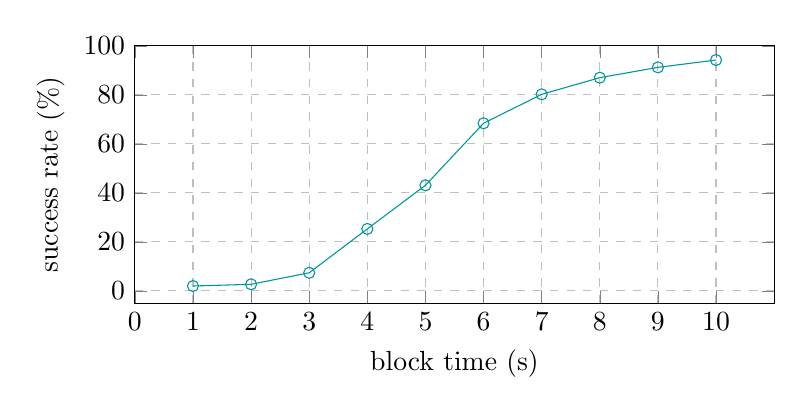
\begin{tikzpicture}
            \definecolor{line-color2}{RGB}{3,150,156}
            \begin{axis}[
                xlabel=block time (s),
                ylabel=success rate (\%),
                xmin=0, xmax=11,
                ymin=-5, ymax=100,
                xtick={0, 1, 2, 3, 4, 5, 6, 7, 8, 9, 10},
                ytick={0, 20, 40, 60, 80, 100},
                grid=major,
                grid style={dashed},
                width=0.8\textwidth,
                height=0.4\textwidth,
            ]

            \addplot[color=line-color2,mark=o] coordinates {
                (1, 2) (2, 2.7) (3, 7.4) (4, 25.3) (5, 43.1) (6, 68.4) (7, 80.2) (8, 87.0) (9, 91.2) (10, 94.2)
            };
            \end{axis}
        \end{tikzpicture}
        \caption{The success rate of the generation of \pol{} certificates, with different block times.}
        \label{fig:block-time-success-rate}
    \end{center}
\end{figure}

In retrospective, the main goal of achieving a fully functional proof-of-concept for the \pol{} protocol was, indeed, achieved. The requirements proposed in Chapter~\ref{sec:protocol-fundamentals} were fulfilled, and a demonstration was made possible. The protocol was implemented in a distributed setting, with a modular network architecture, and a clear separation of concerns between the different stages. The protocol was also engineered with enough flexibility, allowing for an easy integration of new components, or the replacement or tuning of the existing ones, in order to adapt to different environments, or to improve the overall performance. Further measurement considerations, along with the demonstration in a physical environment, are already in the horizon. The next chapter will address the overall conclusions and the future work that may be conducted, in order to improve and expand this \pol{} protocol.

%%%%%%%%%%%%%%%%%%%%%%%%%%%%%%%%%%%%%%%%%%%%%%%%%%%%%%%%%%%%%%%%%%%%%%%%%%%%%%%%

% \begin{figure}[h!]
%     \begin{center}
% \begin{tikzpicture}
%     \definecolor{line-color}{RGB}{92,255,230}
%     \definecolor{line-color2}{RGB}{3,150,156}
%     \begin{axis}[
%         legend pos=outer north east,
%         xlabel=number of instances (witnesses + prover),
%         ylabel=throughput (Kbits/s),
%         xmin=3, xmax=11,
%         ymin=1, ymax=12,
%         xtick={4,5,6,7,8,9,10},
%         ytick={2, 4, 6, 8, 10, 12},
%         grid=major,
%         grid style={dashed},
%         width=0.8\textwidth,
%         height=0.4\textwidth,
%     ]
    
%     \addplot[color=orange,mark=square] coordinates {
%         (4,1.8) (5,3.0) (6,4.2) (7,5.6) (8,7.5) (9,9.0) (10,11)
%         % (4,3.4) (5,5.7) (6,8.1) (7,11.2) (8,14) (9,16.8) (10,20)
%     };
%     % \addlegendentry{batman-adv}

%     % \addplot[color=line-color2,mark=o] coordinates {
%     %     (4,4.5) (5,6.8) (6,9.3) (7,12.7) (8,15.9) (9,19.1) (10,21.8)
%     % };
%     % \addlegendentry{IPv4}

%     \end{axis}
% \end{tikzpicture}
% \caption{Average batman-adv traffic throughput, measured on the bridge interface.}
% \label{fig:mesh-traffic}
% \end{center}
% \end{figure}

% \begin{figure}[h!]
%     \begin{center}
% \begin{tikzpicture}
%     \definecolor{line-color}{RGB}{92,255,230}
%     \definecolor{line-color2}{RGB}{3,150,156}
%     \begin{axis}[
%         legend pos=outer north east,
%         xlabel=number of instances (witnesses + prover),
%         ylabel=throughput (Kbits/s),
%         xmin=3, xmax=11,
%         ymin=2.5, ymax=22.5,
%         xtick={4,5,6,7,8,9,10},
%         ytick={2, 4, 6, 8, 10, 12, 14, 16, 18, 20, 22},
%         grid=major,
%         grid style={dashed},
%         width=0.8\textwidth,
%         height=0.4\textwidth,
%     ]
    
%     \addplot[color=line-color2,mark=o] coordinates {
%         (4,4.5) (5,6.8) (6,9.3) (7,12.7) (8,15.9) (9,19.1) (10,21.8)
%     };
%     \addlegendentry{IPv4}

%     \end{axis}
% \end{tikzpicture}
% \caption{Average batman-adv traffic throughput, measured on the bridge interface.}
% \label{fig:mesh-traffic}
% \end{center}
% \end{figure}

% \begin{figure} [h!]
% \begin{tabular}{c c}
% \begin{minipage}{0.50\textwidth}
%     \begin{center}
%         \begin{tikzpicture}
%             \definecolor{line-color}{RGB}{92,255,230}
%             \definecolor{line-color2}{RGB}{3,150,156}
%             \begin{axis}[
%                 legend pos=outer north east,
%                 xlabel=instances (witnesses + prover),
%                 ylabel=throughput (Kbits/s),
%                 xmin=3, xmax=11,
%                 ymin=1, ymax=12,
%                 xtick={4,5,6,7,8,9,10},
%                 ytick={2, 4, 6, 8, 10, 12},
%                 grid=major,
%                 grid style={dashed},
%                 width=\textwidth,
%                 height=0.8\textwidth,
%             ]
            
%             \addplot[color=orange,mark=square] coordinates {
%                 (4,1.8) (5,3.0) (6,4.2) (7,5.6) (8,7.5) (9,9.0) (10,11)
%                 % (4,3.4) (5,5.7) (6,8.1) (7,11.2) (8,14) (9,16.8) (10,20)
%             };
%             \end{axis}
%         \end{tikzpicture}
%         \caption{(a) Average batman-adv traffic throughput.}
%         % \label{fig:mesh-traffic}
%         \end{center}
% \end{minipage}
% &
% \begin{minipage}{0.50\textwidth}

%     \begin{center}
%         \begin{tikzpicture}
%             \definecolor{line-color}{RGB}{92,255,230}
%             \definecolor{line-color2}{RGB}{3,150,156}
%             \begin{axis}[
%                 legend pos=outer north east,
%                 xlabel=instances (witnesses + prover),
%                 % ylabel=throughput (Kbits/s),
%                 xmin=3, xmax=11,
%                 ymin=2.5, ymax=22.5,
%                 xtick={4,5,6,7,8,9,10},
%                 ytick={2, 4, 6, 8, 10, 12, 14, 16, 18, 20, 22},
%                 grid=major,
%                 grid style={dashed},
%                 width=\textwidth,
%                 height=0.8\textwidth,
%             ]
            
%             \addplot[color=line-color2,mark=o] coordinates {
%                 (4,4.5) (5,6.8) (6,9.3) (7,12.7) (8,15.9) (9,19.1) (10,21.8)
%             };        
%             \end{axis}
%         \end{tikzpicture}
%         \caption{(a) Average IPv4 traffic throughput.}
%         \end{center}

% \end{minipage}
% \end{tabular}
% \caption{Example how to put two figures parallel to each other.}
% \label{fig:LCA_2_solutions}
% \end{figure}

% \begin{figure}[h!]
% \pgfplotstableread[col sep=comma]{data/br-qemu.csv}\datatable

% \begin{tikzpicture}
%     \definecolor{line-color}{RGB}{3,150,156}
%     \definecolor{line-color2}{RGB}{167,169,172}
%     \begin{axis}[
%         xlabel=time (s),
%         ylabel=throughput (Bits/s),
%         xmin=10, xmax=20,
%         ymin=-100, ymax=1300,
%         ytick={0,200,400,600,800,1000,1200},
%         grid=major,
%         grid style={dashed},
%         width=\textwidth,
%         height=0.5\textwidth,
%     ]

%     \addplot[mark=*,line-color2] table[x=Interval start,y=prover 1]{\datatable};
%     \addplot[mark=+,line-color] table[x=Interval start,y=witness 1]{\datatable};
%     \addplot[mark=x,line-color] table[x=Interval start,y=witness 2]{\datatable};
%     \addplot[mark=o,line-color] table[x=Interval start,y=witness 3]{\datatable};

%     \legend{prover, witness 1, witness 2, witness 3}

%     \end{axis}
% \end{tikzpicture}
% \caption{Ethernet traffic throughput, measured on the bridge interface.}
% \label{fig:mesh-traffic-3-witnesses}
% \end{figure}


% \begin{figure}[h!]
% \pgfplotstableread[col sep=comma]{data/blockchain-blocks-generation-8-instances.csv}\datatable

% \begin{tikzpicture}
%     \definecolor{line-color}{RGB}{3,150,156}
%     \definecolor{line-color2}{RGB}{167,169,172}
%     \begin{axis}[
%         xlabel=time (s),
%         ylabel=messages,
%         xmin=-2, xmax=102,
%         ymin=-50, ymax=300,
%         ytick={0, 50, 100, 150, 200, 250, 300},
%         grid=major,
%         grid style={dashed},
%         width=\textwidth,
%         height=0.5\textwidth,
%         legend pos=north west
%     ]

%     \addplot[mark=*,line-color] table[x=x,y=TCP]{\datatable};
%     \addplot[mark=+,line-color2] table[x=x,y=UDP]{\datatable};
%     \addplot[mark=o,orange] table[x=x,y=Batman-adv-orig]{\datatable};

%     \legend{TCP, UDP, Batman-adv-orig}

%     \end{axis}
% \end{tikzpicture}
% \caption{The network activity, with a block time of 10 seconds.}
% \label{fig:blockchain-blocks-generation}
% \end{figure}


% AMD Ryzen 7 4700U with Radeon Graphics (with SSE4.2)
% Linux 6.1.24-1-lts
